\subsection{Técnicas de estimación de la posición}

Existen dos alternativas para estimar la posición de un objetivo a partir de la posición conocida de un cierto número de balizas con coordenadas conocidas: la primera, denominada \textit{fingerprinting} se basa en la obtención de un modelo de posicionamiento a partir de la medición de la potencia de las balizas; la segunda, obtiene las estimaciones a partir de técnicas geométricas \cite{MAIN}.

\subsubsection{\textit{Fingerprinting}}

La primera de las opciones para estimar la posición de un objetivo se basa en la medición de la potencia de la señal recibida desde cada una de las balizas.

Esta técnica requiere un mapeado previo de la zona de interés que permita obtener un modelo contra el que comparar en su uso posterior.
La dependencia en un modelo previo provoca que cualquier modificación del entorno --como por ejemplo tránsito de personas-- hace que la estimación sea en el mejor de los casos ligeramente distinta y en el peor, imposible.

La comparación contra el modelo hace uso de algoritmos de \textit{machine learning} como \textit{k-nearest-neighbor} o \textit{support vector regression}, que buscan minimizar la diferencia entre las medidas y dicho modelo. 
Requieren, de forma general, una capacidad computacional mayor a las alternativas geométricas, por lo que son usados habitualmente en entornos con obstáculos estáticos y sin demasiadas modificaciones, donde su ventaja es significativa.

\subsubsection{Técnicas geométricas}

La multiliteración -- también llamada \textit{triliteración} en el caso de usar tres puntos de referencia -- es una técnica para conocer la posición de un objetivo con argumentos geométricos.

Se basa en la búsqueda de la intersección de las áreas de distancia conocida a partir de la posición de varias balizas.
Estas áreas están definidas por distancias o ángulos a las balizas de referencia, valor obtenible con distintas técnicas.

En general, la posición del objetivo vendrá dado, en $n$ dimensiones, por
\begin{equation}\label{eq:geom}
    \vb{r} = \vb{f}(x_1, x_2, \ldots, x_n) + \vb{n}
\end{equation}
donde $\vb{f}$ será la función característica de cada algoritmo y $\vb{n}$ un vector con el ruido de la señal, con un valor medio nulo.

% \subsubsubsection{Límites teóricos}

% Al plantear la ecuación general de las técnicas geométricas \eqref{eq:geom} se introdujo un término relacionado con el ruido relacionado con la generación y el traslado de la señal desde la baliza hasta el objetivo.
% Este ruido tiene un carácter aleatorio, por lo que su caracterización habitual es la de ruido blanco gaussiano, con valor medio cero.

Este ruido está relacionado con la generación y el traslado de la señal desde la baliza hasta el objetivo y tiene un carácter aleatorio, por lo que su caracterización habitual es la de ruido blanco gaussiano, con valor medio cero.

Esta caracterización, unida al muestreo discreto de la señal por parte de los dispositivos electrónicos resulta en un límite en la precisión del posicionamiento, incluso en los casos más ideales.

El límite más usual viene dado por la cota inferior de Cramer-Rao (CRLB), definido como la traza de la matriz de Fisher inversa.
La matriz de Fisher se construye, en el caso de la parametrización del ruido con características gaussianas, como \cite{Xbook}
\begin{equation}
    [\mathcal{I}(\bm{\theta})]_{ij} = \frac{1}{\sigma^2} \sum_{n=0}^{N=1} \pdv{s[n,\bm{\theta}]}{\theta_i}\pdv{s[n,\bm{\theta}]}{\theta_j}
\end{equation}
donde $\bm{\theta}$ indica el vector con los parámetros a evaluar, $\sigma$ la desviación del ruido blanco gaussiano, $N$ el número de balizas utilizadas y $s[n,\bm{\theta}]$ la señal emitida por la baliza $n$, sin ningún ruido.

Así, la varianza de cada uno de los parámetros a estimar vendrá dada como
\begin{equation}
    \sigma^2(\theta_i) \geq [\mathcal{I}(\bm{\theta})^{-1}]_{ii}
\end{equation}

% Así, se obtiene un límite para cada tipo de técnica, ya que se medirán distintos parámetros en cada una de ellas, dados por:
% \begin{equation}
%     \text{CRLB}
%     \begin{cases}
%         \displaystyle\frac{1}{8\pi^2 \text{SNR} \beta^2} & \text{TOA y TDOA} \\
%         \\[2pt]
%         \displaystyle\frac{1}{2\pi^2 \text{SNR} \beta^2 N(N^2-1)d\cos(\theta)} & \text{AOA} \\
%         \\[2pt]
%         \displaystyle\frac{\ln(10)\sigma_{sh}d}{10n} & \text{RSSI} \\
%     \end{cases}
% \end{equation}
% donde $\beta$ denota el ancho de banda efectivo dado por
% \begin{equation}
%     \beta^2 = \frac{\int_{-\infty}^{\infty} \omega^2 \abs{S(\omega)}^2\dd{\omega}}{\int_{-\infty}^{\infty} \abs{S(\omega)}^2\dd{\omega}}
% \end{equation}
% con $S(\omega)$ como la transformada de Fourier de la señal $s(t)$.

% SNR es la razón entre la señal y el ruido --\textit{signal-to-noise ratio}, en inglés--, de la que se tiene una relación inversamente proporcional.

% Para los casos de AOA y TOA, el CRLB toma valores demasiado bajos cuando el SNR es muy bajo.
% Por ello en dichas situaciones es habitual el uso de la cota inferior de Ziv-Zakai (ZZLB) \cite{soganzi}, que no sufre este problema, aunque no siempre es posible evaluar de forma analítica.

% Con argumentos geométricos es posible construir una serie de algoritmos basados en la posición conocida de ciertas balizas.

\subsubsubsection{Tiempo de llegada (TOA)}

El primer algoritmo considera una velocidad de transmisión conocida y una línea de visión directa entre las balizas y el objetivo.
Teniendo en cuenta que el medio de propagación será aire, la velocidad de la señal será la velocidad de la luz en el caso de ondas electromagnéticas.
Esta velocidad no tendrá variaciones significativas al cambiar la zona de interés, por lo que será válida para prácticamente cualquier escenario.

Denotando al objetivo como OBJ y con tres balizas llamadas $B_i$ con $i=1,2,3$, la distancia recorrida por cada señal hasta el objetivo será \footnote{Durante todo el desarrollo de la teoría de posicionamiento en esta sección se supondrá un sistema bidimensional. Esto no puede ser así en la implementación \textit{real}, pero teniendo en cuenta que en el posicionamiento local se trata con sistemas euclídeos la adición de la tercera componente en todos los cálculos es trivial.}
\begin{equation}\label{eq:TOA}
    \begin{aligned}
        d_i &= c(t_i) = c(\tau_i - t_0) \\
        &= \sqrt{(x_i - x)^2 + (y_i - y)^2} + ct_0
    \end{aligned}
\end{equation}
siendo $t_0$ el instante en el que la baliza $i$ emitió el pulso.
Así, la función característica de este algoritmo será, en dos dimensiones
\begin{equation}
    f_i(x, y) = \sqrt{(x_i - x)^2 + (y_i - y)^2}
\end{equation}
para cada baliza.

\begin{figure}[H]
    \centering
    \def\svgwidth{0.6\linewidth}
    \input{./fig/TOA.pdf_tex}
	\caption{Posicionamiento por tiempo de vuelo (TOA).}
    \label{fig:TOA}
\end{figure}

A partir de las ecuaciones de \eqref{eq:TOA} la posición de OBJ será \cite{Zafer}
\begin{equation}
    \begin{aligned}
        x = \frac{(y_2-y_1)\gamma_1 + (y_2-y_3)\gamma_2}{2[(x_2-x_3)(y_2-y_1) + (x_1 - x_2)(y_2 - y_3)]}\\
        y = \frac{(x_2-x_1)\gamma_1 + (x_2-x_3)\gamma_2}{2[(x_2-x_1)(y_2-y_3) + (x_2 - x_3)(y_1 - y_2)]}\\
    \end{aligned}
\end{equation}
donde
\begin{equation}
    \begin{aligned}
        \gamma_1 = x_2^2 - x_3^2 + y_2^2 - y_3^2 + d_3^2 - d_2^2 \\
        \gamma_2 = x_1^2 - x_2^2 + y_1^2 - y_2^2 + d_2^2 - d_1^2 \\
    \end{aligned}
\end{equation}

En este algoritmo es crítica una correcta sincronización entre los relojes de las balizas y el objetivo.
Es posible minimizar este problema usando solo uno de los puntos para medir la distancia esperando una reemisión: emitiendo, desde una de las balizas o el objetivo, un pulso y esperando una respuesta similar del objetivo, con lo que el tiempo total será el doble del tomado por la señal original en llegar a la posición requerida.

El CRLB en el caso de TOA viene dado por \cite{Xbook}
% Esta precisión vendrá por tanto dada por el nivel de ruido en la señal, con la expresión
\begin{equation}\label{eq:CRLB_TOA}
    \text{CRLB} = \sigma^2(\tau) \geq \frac{1}{8\pi^2\text{SNR}\beta^2}
\end{equation}
donde $\tau$ es la distancia estimada y $\beta$ el ancho de banda efectivo dado por
\begin{equation}
    \beta^2 = \frac{\int_{-\infty}^{\infty} \omega^2 \abs{S(\omega)}^2\dd{\omega}}{\int_{-\infty}^{\infty} \abs{S(\omega)}^2\dd{\omega}}
\end{equation}
con $S(\omega)$ como la transformada de Fourier de la señal $s(t)$.

SNR es la razón entre la señal y el ruido --\textit{signal-to-noise ratio}, en inglés--, de la que se tiene una relación inversamente proporcional.
Es decir, la relación esperada: el SNR proporciona la relación entre la energía de la señal y la energía del ruido que la corrompe, así que un valor mayor indica menos ruido y por tanto una incertidumbre menor en la intersección de los pulsos de las balizas.

En este caso, el CRLB toma valores demasiado bajos cuando el SNR es muy bajo.
Por ello en dichas situaciones es habitual el uso de la cota inferior de Ziv-Zakai (ZZLB) \cite{soganzi}, que no sufre este problema, aunque no siempre es posible evaluar de forma analítica.

\subsubsubsection{Diferencia de tiempo de llegada (TDOA)}

Para eliminar la sincronización de relojes entre las balizas y el objetivo es posible usar también la diferencia temporal entre las señales de las balizas, teniendo así independencia en el sistema del objetivo.
Aunque se consiga la independencia del reloj del objetivo, esta configuración sigue requiriendo que los relojes de las balizas estén sincronizados entre sí.

Así, la diferencia entre las distancias de las señales de dos balizas, teniendo en cuenta los tiempos en la llegada de la señal de dos balizas será
\begin{equation}\label{eq:TDOA}
        d_{ij} = c(t_i - t_j) = c \left[  (\tau_i + t_0) - (\tau_j + t_0)\right] = c(\tau_i - \tau_j)
\end{equation}
válida para $i=1,2,3$ y $j=1,2,3$ con $i \neq j$.
Así, la función característica de este algoritmo será
\begin{equation}
    f_i(x,y) = \sqrt{(x_i - x)^2 + (y_i - y)^2} - \sqrt{(x_j - x)^2 + (y_j - y)^2}
\end{equation}
para cada baliza $i$ respecto de cualquiera $j$ de las otras.

\begin{figure}[H]
    \centering
    \def\svgwidth{0.6\linewidth}
	\input{./fig/TDOA.pdf_tex}
	\caption{Posicionamiento por diferencia tiempo de vuelo (TDOA)}
\end{figure}
Así, tomando la baliza 1 como referencia tenemos que las coordenadas del objetivo vienen dadas por el sistema de ecuaciones
\begin{equation}
    \begin{cases}
        d_{12} &= \sqrt{(x_1 - x)^2 + (y_1 - y)^2} - \sqrt{(x_2 - x)^2 + (y_2 - y)^2} \\
        d_{13} &= \sqrt{(x_1 - x)^2 + (y_1 - y)^2} - \sqrt{(x_3 - x)^2 + (y_3 - y)^2} \\
    \end{cases}
\end{equation}
con el que se obtiene de forma general dos soluciones para el posicionamiento: en la mayoría de casos una de ellas será un punto fuera de los límites del recinto en que se trabaja por lo que se elegirá el más cercano a las balizas colocadas.

En el caso de TDOA el CRLB tiene la misma expresión que en el TOA \eqref{eq:CRLB_TOA}, teniendo en cuenta que el ruido añadido a las señales de las balizas tendrá la misma caracterización.

\subsubsubsection{Intensidad de la señal recibida (RSSI)}

Para evitar problemas con la sincronización de los relojes necesaria en las técnicas anteriores es posible aprovechar el decaimiento de la intensidad de la señal con la distancia según la relación
\begin{equation}\label{eq:RSSI}
    p(r) = p(r_0) - 10n\log(\frac{r}{r_0})
\end{equation}
donde $p(r_0)$ y $p(r)$ son la intensidad de la señal en el origen y el objetivo respectivamente y $n$ el exponente de atenuación de la señal.

Esta técnica es muy susceptible ante el ruido ambiental y las posibles interferencias que puedan ocurrir entre las señales de distintas balizas o de fuentes externas.
La disposición geométrica es similar a la vista en la técnica de tiempo de llegada (Fig \ref{fig:TOA}), donde a partir de una medición de la señal de una baliza es posible definir una circunferencia de centro en dicha baliza y radio dado por \eqref{eq:RSSI}.

A diferencia de los casos de TOA y TDOA el CRLB en esta técnica es independiente del ancho de banda de la señal, dado por \cite{MAIN}
\begin{equation}\label{eq:CRLB_RSSI}
    \sigma^2(d_i) = \frac{\ln(10)\sigma_{sh}d}{10n}
\end{equation}
donde $\sigma_{sh}$ indica la desviación estándar del desvanecimiento de la señal.

La independencia de las cotas inferiores del ancho de banda de la señal hacen que esta técnica no aproveche la principal ventaja que da el UWB, por lo que su uso se restringe a otras tecnologías.

\subsubsubsection{Ángulo de llegada (AOA)}

Otra opción para evitar la sincronización de los relojes entre las balizas consiste en usar el ángulo de incidencia de la señal en el objetivo, de tal forma que, para una baliza $B_i$ dicho el objetivo se encuentra en la posición
\begin{equation}
    \label{eq:AOA}
    \begin{aligned}
        x = d_i \cos(\phi_i) + x_i \\        
        y = d_i \sin(\phi_i) + y_i         
    \end{aligned}
\end{equation}
por lo que la función característica de este algoritmo será la distancia de cada baliza al objetivo, a partir de \eqref{eq:AOA}
\begin{equation}
    f_i = \arctan(\phi_i) = \arctan(\frac{y-y_i}{x-x_i})
\end{equation}

\begin{figure}[H]
    \centering
    \def\svgwidth{0.6\linewidth}
	\input{./fig/AOA.pdf_tex}
    \caption{Posicionamiento por ángulo de llegada (AOA).}
    \label{fig:AOA}
\end{figure}
Esta técnica requiere el uso de antenas direccionales, lo que hace que aumente el coste de su implantación.

En este caso solo necesitamos el ángulo respecto a las balizas, por lo que su implantación será más adecuada en situaciones en las que el cálculo de la distancia entre objetivo y balizas no es fiable o como apoyo o correción junto con TOA o TDOA.

Para el AOA el CRLB, que nos dará el mínimo de varianza para el ángulo de incidencia vendrá dado, en el caso de balizas colocadas a lo largo de un eje de la forma mostrada en la Figura~\ref{fig:AOA} por \cite{Xbook, shim2018}
\begin{equation}
    \sigma^2(\phi) = \frac{c^2}{2\pi^2 \text{SNR} \beta^2 N(N^2-1)d\cos(\phi)}
\end{equation}
donde $N$ indica el número de balizas utilizadas y $d$ la distancia entre ellas.

\subsubsection{Mitigación en casos no ideales}

En el planteamiento de los algoritmos geométricos se suponía una línea de visión directa entre las balizas y el objetivo para determinar los parámetros de interés, pero en condiciones reales esta suposición no siempre podrá ser respetada.

La presencia de obstáculos que impidan un trayecto de la señal parametrizable o generen rebotes en la zona de interés pueden provocar un posicionamiento erróneo o, en el peor de los casos, imposible.

Para mitigar la modificación en la señal en estos casos se recurre a técnicas estadísticas que se dividen en dos grupos: técnicas paramétricas, en las que se realiza un ajuste del error a una distribución de probabilidad conocida, y técnicas no paramétricas, en la que no se asume ninguna distribución a priori.

% \subsubsubsection{Técnicas paramétricas}

% El primer grupo de técnicas consiste en aplicar argumentos estadísticos de tal forma que es posible ajustar la señal recibida en el objetivo a una cierta función de probabilidad, de tal manera que es posible filtrar en cierta medida el ruido y las interferencias que acompañan al pulso original \cite{Zafer}.

% Definiendo como $\bm{\theta} = [x,y,\lambda]^T$ el vector que contiene los parámetros de la distribución, podemos establecer una función de probabilidad del ruido introducido en la señal como
% \begin{equation}
%     p(r|\bm{\theta})
% \end{equation}
% indicando la probabilidad de densidad de $r$ conociendo $\bm{\theta}$.

% A partir de esta función de probabilidad es posible aplicar estimadores Bayesianos, principalmente el mínimo error cuadrático medio (MMSE, \textit{minimum mean square error}) definido como
% \begin{equation}\label{eq:MMSE}
%     \hat{\bm{\theta}}_{\text{MMSE}} = E\{\bm{\theta}|\vb{r}\}
% \end{equation}
% con $E\{\bm{\theta}|\vb{r}\}$ como el valor esperado de $\bm{\theta}$ dado $\vb{r}$, o el estimador de máximos a posteriori (MAP), definido como
% \begin{equation}
%     \hat{\bm{\theta}}_{\text{MAP}} = \argmax_{\bm{\theta}} p(\bm{\theta}|r)
% \end{equation}

% A partir del teorema de Bayes tenemos que
% \begin{equation}
%     p(\bm{\theta}|r) = \frac{p(r|\bm{\theta})p(\bm{\theta})}{p(r)}
% \end{equation}
% por lo que maximizar $p(\bm{\theta}|r)$ equivale a maximizar $p(r|\bm{\theta})p(\bm{\theta})$ y así tenemos que la estimación a posteriori será \cite{Xbook}
% \begin{equation}\label{eq:MAP}
%     \hat{\bm{\theta}}_{\text{MAP}} = \argmax_{\bm{\theta}} p(r|\bm{\theta})p(\bm{\theta})
% \end{equation}
% o de forma equivalente
% \begin{equation}
%     \hat{\bm{\theta}}_{\text{MAP}} = \argmax_{\bm{\theta}} [\ln(p(r|\bm{\theta})) + \ln(p(\bm{\theta})) ]
% \end{equation}
% con $p(\bm{\theta})$ como la información a priori de la distribución de probabilidad del ruido de la señal.

% En el caso de las señales utilizadas, dicha distribución a priori es a veces exponencial si en el camino recorrido se espera un gran número de obstáculos o, de forma más habitual, de tipo gaussiano.

% En los casos en los que esta información a priori no es conocida es posible utilizar un estimador por máxima similitud de tal forma que la estimación será
% \begin{equation}\label{eq:ML}
%     \hat{\bm{\theta}}_{\text{ML}} = \argmax_{\bm{\theta}} p(r|\bm{\theta})
% \end{equation}
% donde la función de similitud vendrá dada por
% \begin{equation}
%     p(r|\bm{\theta}) = p_n(\vb{r} - \vb{f}|\bm{\theta})
% \end{equation}
% a partir de \eqref{eq:geom}.
% $p_n(\cdot | \bm{\theta})$ indica la función de probabilidad del vector de ruido condicionada por los parámetros de $\bm{\theta}$.

% En el caso de componentes de ruido independientes esta función de probabilidad será
% \begin{equation}
%     p_n(\vb{r} - \vb{f}|\bm{\theta}) = \prod_i^{N} p_{n_i}(r_i - f_i|\bm{\theta})
% \end{equation}
% donde, como en el caso de la estimación a posteriori, la parametrización habitual es la de una distribución gaussiana para cada componente.

% Esta asunción es generalmente válida en el caso de TOA, AOA o RSS, donde el ruido de cada baliza no interferirá en los otros.
% No será el caso de las estimaciones con TDOA, donde en el cálculo de los parámetros de interés intervendrá el ruido generado en la señal de al menos dos balizas, por lo que es necesario establecer una mínima correlación.

% Cabe recordar que en los casos ideales ya se tenía en consideración un cierto ruido en el transporte de la señal.
% En los casos no ideales tratados ahora --como puede ser por ejemplo la presencia de obstáculos-- no se deja de considerar aquella primera aproximación, por lo que las funciones de probabilidad tratadas en total tendrán dos componentes: el del caso ideal más una nueva componente fruto del nuevo entorno.

% \subsubsection{Técnicas no paramétricas}

% En los casos en los que no es posible conocer una distribución a priori del ruido ni modelizarlo con una cierta distribución de probabilidad se recurre habitualmente a un ajuste de mínimos cuadrados.
% Así, definiendo $\vb{z} = [x,y]^T$ como la posición desconocida del objetivo, $\vb{z}_i$ la posición de la baliza $i$ y $r_i$ la distancia obtenida entre el objetivo y dicha baliza se tiene \cite{MAIN}
% \begin{equation}
%     \hat{\vb{z}} = \argmin_{\vb{z}} \sum_i(r_i - ||\vb{z} - \vb{z}_i||)^2
% \end{equation}
% con $||\vb{z} - \vb{z}_i||$ como el módulo euclídeo indicando la distancia entre cada baliza y el objetivo.

% En el caso de mediciones con TDOA este módulo debe ser modificado para adecuarse a la naturaleza hiperbólica de la curvas de las que se busca la intersección.

% En condiciones reales los ajustes de mínimos cuadrados se ven muy contaminados por los escenarios sin visión directa y las incertidumbres de los sensores, por lo que habitualmente se usan ciertos pesos en las medidas de cada una de las balizas para favorecer a aquellas en las que la recepción es más favorable.

\subsection{Tecnologías}

Todos los algoritmos geométricos mencionados necesitan un soporte físico para determinar las variables posicionales del objetivo que requieren, para lo que es posible el uso de varias tecnologías, como se recoge en \cite{COMP}, de donde procede toda la información de esta sección.

\subsubsection{Sonido}

Una primera propuesta puede ser el uso de ondas de sonido, normalmente fuera del rango de audición humano. Dependiendo de la frecuencia utilizada son referidos a veces como \text{ultrasonidos}.

La baja velocidad de propagación en el aire hace que la incertidumbre en la medida de los tiempos de llegada sea muy baja, por lo que su uso se asocia casi exclusivamente a TOA y TDOA.

Esta tecnología tiene su principal punto débil en la dependencia de la propagación del sonido con la temperatura y la humedad del aire: la precisión ganada por la baja velocidad de propagación se ve compensada con un rango máximo muy bajo, lo que hace que su implantación en entornos amplios no sea óptimo.
Además, el equipamiento necesario tiene un coste mayor al de sus alternativas, por lo que su uso se restringe actualmente a situaciones concretas.

\subsubsection{Luz}

La popularización de la iluminación LED, capaz de cambiar la intensidad de emisión en tiempos muy cortos ha provocado el desarrollo de tecnologías que modulen información a tasas de tiempo mucho más altas de la que el ojo humano puede captar.

Su principal ventaja es la posibilidad de aprovechar las infraestructuras de iluminación ya existentes en ambientes interiores, aunque esta tecnología es muy dependiente de las condiciones en dichas situaciones.

La desventaja más directa es su total reflexión en paredes u objetos opacos, lo que hace que la atenuación sea importante en interiores donde la disposición desfavorezca una iluminación uniforme o simplemente un tráfico intenso de personas.
Además, es muy sensible a fuentes externas como luz solar.

\subsubsection{Visión por computador}

El desarrollo en los últimos años de técnicas para el reconocimiento de imágenes ha hecho posible la obtención de técnicas de posicionamiento con cámaras.

Esta técnica ha tenido especial auge en el campo de vehículos autónomos, aunque su uso se complementa de forma habitual con otras tecnologías al necesitar buenas condiciones lumínicas para su correcto funcionamiento.

Al igual que en el caso de la luz, su principal ventaja reside en el aprovechamiento de la infraestructura ya existente.
En este caso es posible utilizar una tecnología ya asentada y madura sin realizar ninguna modificación sin más que usar cámaras con la resolución suficiente para los distintos casos de uso.

\subsubsection{Campo magnético}

Aunque hay algunos trabajos que desarrollan el sistema de posicionamiento sobre un campo magnético artificial, la mayoría de aplicaciones se basan en el campo magnético terrestre para determinar la posición del objetivo.

Estas técnicas requieren un estudio previo para determinar la intensidad de dicho campo magnético terrestre a lo largo del espacio en los que implementar el posicionamiento, aunque tras ello el equipamiento necesario es mínimo al requerir únicamente un magnetómetro.

Este tipo de técnicas tiene una precisión muy baja, en torno a metros, y es muy susceptible a cualquier modificación del campo magnético sobre el que se realizó el estudio previo por lo que su aplicación se reduce a situaciones muy concretas.

\subsubsection{Wi-Fi}

En el espectro electromagnético las señales de Wi-Fi son también una alternativa a la hora de determinar distancias por el decaimiento de su intensidad con la distancia.
Su atractivo principal es, como en otras tecnologías, el aprovechamiento de las infraestructuras y el desarrollo ya existente.

Aunque también es posible su uso con TOA y AOA, su uso principal se restringe a técnicas de \textit{fingerprinting}, ya que habitualmente los puntos de acceso Wi-Fi usados para la conexión a internet no suelen superar la unidad por planta o edificio.

Esta escasez de balizas es la principal desventaja: en su uso original un solo emisor puede dar servicio a multitud de dispositivos en una planta o incluso un edificio, por lo que lo habitual será encontrar numerosos obstáculos entre emisor y objetivo.
Colocar más balizas puede añadir interferencias entre las señales teniendo en cuenta que los canales disponibles tienen un ancho de banda bajo.

Además, el uso extendido de esta tecnología inalámbrica hace que su espectro esté ya, en algunas ocasiones, saturado.
Su precisión en ambientes ideales está en torno al metro, así que podría ser una buena opción en entornos abiertos o con pocas redes que puedan causar interferencias.

\subsubsection{Bluetooth}

En el caso del Bluetooth nos encontramos de nuevo con una tecnología con una gran infraestructura ya existente teniendo en cuenta que su uso en teléfonos móviles se da desde hace más de una década.

Entre las distintas generaciones se encuentra un protocolo llamado Bluetooth Low Energy (BLE) centrado en obtener un funcionamiento con el mínimo gasto energético posible, lo que lo hace idóneo para usar como sistema para localización como el que se trata en este trabajo.

Técnicamente comparte el mismo rango de frecuencias con el Wi-Fi y las técnicas de posicionamiento son en general parecidas, aprovechando el decaimiento de la señal con técnicas de \textit{fingerprinting}.
Pero a diferencia del Wi-Fi, la baja energía de los emisores BLE permiten la colocación de un número mayor de balizas, lo que abre la puerta al uso de algoritmos de multiliteración.

Los mejores resultados sobre esta tecnología arrojan una precisión entre 1 y 3 metros, aunque estos resultados dependen en gran medida del número de balizas empleadas.

\subsubsection{Otras tecnologías}

Además de los soportes físicos ya mencionados, existe un enorme abanico de otras tecnologías.
La más ampliamente usada y no mencionada se encuentra en el espectro electromagnético dedicado a las redes móviles, aunque las grandes distancias a las que se encuentran las balizas --torres de comunicación en este caso-- hace que la precisión, en las mejores ocasiones, se encuentre en torno a los 50 metros, inviable para una localización en interiores.

Es posible que el desarrollo de nuevas generaciones de este tipo de redes como el 5G permitan tener una mayor precisión para permitir su uso.

Entre otras alternativas se encuentran también de comunicaciones a muy corta distancia como el \textit{Near-Field Communication} (NFC), aunque este sistema requiere una participación activa del objetivo --debe acercarse mucho a alguna de las balizas-- y no permite localización de objetos en movimiento.

\subsection{Ultra-Wide Band}

El Ultra-Wide Band (UWB) se define como una emisión de radiofrecuencia con un ancho de banda de al menos 500 MHz o más del 20\% de la frecuencia central.
Su definición técnica se recoge en el estándar 802.15.4 del IEEE junto con otras redes inalámbricas de área personal.

Los canales usados y las potencias permitidas tienen distintas legislaciones según el país que se trate.
En el caso de Europa, la regulación del Instituto Europeo de Normas de Telecomunicaciones (ETSI) permite emisiones en los rangos de frecuencia $3.1 - 4.8\si{\giga\hertz}$, destinado a localización de servicios de emergencia y  $6.0 - 9.0\si{\giga\hertz}$ para localización general \cite{UWB_regs}.

\subsubsection{Ventajas}

La principal característica del UWB, su gran ancho de banda, le da varias ventajas en su uso principal y que se discute en este trabajo: servicios de localización a partir de técnicas geométricas.
Aunque sea el principal uso no es el único, ya que también permite transmisión de datos de una forma rápida y puede ser una alternativa en este tipo de situaciones.

El espectro tan amplio de frecuencia provoca que el decaimiento de la señal, dependiente de la frecuencia, sea fácilmente identificable al estar formado de componentes que sufren este hecho de forma acusada.

En el caso de que se produzca propagación multicamino, en la que los rebotes creen nuevos frentes de onda, la resolución del camino principal se vuelve sencilla teniendo en cuenta que el espacio adicional que recorran las trayectoria sin visión directa --fruto de la reflexión en paredes u obstáculos-- hacen que estos caminos secundarios se verá rápidamente desfavorecidos.

Además, el amplio ancho de banda hace que las interferencias entre los propios pulsos fruto de los distintos caminos sean mínimas, nulas si el tiempo de propagación adicional supera el periodo entre la emisión de dos pulsos.

Este último hecho es muy probable en el caso del UWB.
El tiempo de transmisión de un pulso viene dado por\cite{MAIN}
\begin{equation}
    T_{tx} = \left(N_d + \frac{N_d}{N_{mP}N_{0}N_d} \right) T_b T_{pr}
\end{equation}
donde $N_d$, $N_{mP}$ y $N_{0}$ indican los tamaños de datos, tasa máxima y \textit{overhead} respectivamente;
mientras que $T_b$ y $T_{pr}$ indican la duración y el tiempo de propagación de cada bit, respectivamente.

Si el tiempo de propagación es inversamente proporcional a la tasa de datos, muy amplia en el caso del UWB, el tiempo de propagación será por tanto muy bajo, lo que no solo evita las interferencias sino que permite una resolución temporal muy alta.

La tasa de datos viene dada por capacidad de un canal, dada en bits/sec como\cite{MAIN}
\begin{equation}
    C = B\log_2(1 + \text{SNR})
\end{equation}
siendo $B$ el ancho de banda de dicho canal y considerando ruido blanco gaussiano en el transporte de la señal.

Esta gran capacidad es la que convierte al UWB una de las mejores alternativas para el transporte de datos, aunque su adopción en este ámbito no es hasta el momento demasiado amplia.

Otra de las características del UWB es su eficiencia energética.
Aunque es posible entender este término de distintas formas, a la hora de realizar comparaciones se suele recurrir a la capacidad por unidad de potencia o al tiempo de uso permitido con sensores alimentados con baterías.

La gran capacidad de transmisión de los canales de UWB hace posible jugar con el periodo de emisión de los pulsos, lo que permite un consumo menor.
Por ello, la densidad de energía espectral es muy baja con tasas de transmisión altas; así, la capacidad de detección de estas emisiones es complicada, lo que abre la puerta a aplicaciones militares.

Esta baja densidad de energía espectral también hace que las interferencias con canales con ancho de banda menor tengan un efecto mínimo.
Un gran ancho de banda permite el uso de varias bandas del espectro electromagnético a la vez, por lo que el uso en ambientes con señales de Wi-Fi o Bluetooth --tecnologías con un ancho de banda estrecho-- es posible.
Aun así, es habitual el uso de técnicas de detección y evasión (DAA), en las que antes de la puesta en marcha de la transmisión se evalúan los canales en uso para evitar en la medida de lo posible las bandas ya ocupadas.

\subsubsection{Pulsos de UWB}

En el diseño de sistemas de UWB la elección de la forma del pulso es crucial, ya que determina la respuesta en frecuencias como se muestra en la Figura~\ref{fig:Pulsos}.
Los pulsos mayoritariamente tienen perfiles gaussianos, aunque con distintas características \cite{Du}.

La primera opción es el uso de una forma gaussiana clásica
\begin{equation}\label{eq:pulso_gauss}
    y(t) = A\exp(-a^2 t^2)
\end{equation}
donde $A$ indica la máxima amplitud del pulso y $a$ la constante que indica la pendiente del pulso por lo general elegida de modo que el pulso tenga una duración en el orden de centenas de picosegundos o nanosegundos.

Su respuesta espectral, dada por la transformada de Fourier será    
\begin{equation}
    Y(\omega) = \frac{A}{a\sqrt{2}}\exp(-\frac{\omega^2}{4a})
\end{equation}
con pico en $f_0=0$, a partir del cual es posible determinar el ancho de banda teniendo en cuenta que debe ser 3dB menor que dicho pico como
\begin{equation}
    \Delta f = 0.8326\frac{a\sqrt{2}}{2\pi}
\end{equation}

La segunda opción, llamada gaussiana monocíclica, consiste en la primera derivada temporal de \eqref{eq:pulso_gauss}
\begin{equation}
    y(t) = -2 a^2 At\exp(-a^2 t^2)
\end{equation}
con la respuesta espectral
\begin{equation}
    Y(\omega) = \frac{i\omega A}{a\sqrt{2}}\exp(-\frac{\omega^2}{4a})
\end{equation}
con frecuencia máxima
\begin{equation}
    f_0 = \frac{a\sqrt{2}}{2\pi}
\end{equation}
y ancho de banda
\begin{equation}
    \Delta f = 1.155\frac{a\sqrt{2}}{2\pi}
\end{equation}

Este pulso suele ser el utilizado para el diseño de los sistemas de UWB.
A diferencia del pulso gaussiano simple, este pulso tiene un nodo con amplitud cero, lo que elimina las posibles componentes contínuas y añaden una referencia en la señal, además de una menor energía en señales de baja frecuencia, transmitidas de forma muy ineficiente por las antenas de los emisores de UWB.

Es también idónea teniendo en cuenta las técnicas de modulación de la información usadas, para las que se necesita una referencia en la amplitud del pulso o una forma característica que sea posible invertir.

Por último es posible tomar la segunda derivada de \eqref{eq:pulso_gauss} para llegar al pulso gaussiano de doblete, caracterizado como
\begin{equation}
    y(t) = -2 a^2 A\exp(-a^2 t^2)(1 - 2a^2 t^2)
\end{equation}
con respuesta espectral
\begin{equation}
    Y(\omega) = \frac{-\omega^2 A}{a\sqrt{2}}\exp(-\frac{\omega^2}{4a})
\end{equation}
con frecuencia máxima
\begin{equation}
    f_0 = \frac{a}{\pi}
\end{equation}
y ancho de banda
\begin{equation}
    \Delta f = 1.155\frac{a\sqrt{2}}{2\pi}
\end{equation}
igual que en el caso monocíclico aunque con frecuencia central distinta.

Este pulso tiene características muy parecidas al monocíclico: un ancho de banda similar y la ausencia de posibles componentes de corriente continua al contar ahora con dos puntos donde la amplitud es nula.

La principal diferencia radica en la frecuencia en la que se da la respuesta máxima, ahora con un valor más alto.
Sucesivas derivaciones de \eqref{eq:pulso_gauss} tendrán el mismo resultado, con igual ancho de banda y valores crecientes de $f_0$, por lo que este tipo de pulsos de mayor orden es quizá adecuado para canales cercanos al límite superior del espectro \cite{design}.

\begin{figure}[H]
\begin{tikzpicture}
    \centering
    \pgfplotsset{footnotesize,samples=100}
    \begin{groupplot}[group style = {group size = 2 by 1, horizontal sep = 45pt},
            xmajorgrids, ymajorgrids,
            width = 0.5\textwidth, height = 0.4\textwidth,]
        \nextgroupplot[
                % title = {Tiempo},
                legend style = { column sep = 10pt, legend columns = -1, legend to name = grouplegend,},
                xtick={-0.4, -0.3,...,0.4}, ytick={1,0.5,...,-1},
                xmin = -0.35, xmax=0.35,
                xlabel={Tiempo (ns)},
                ylabel={Amplitud}]
            \addplot[red, dashed, very thick, domain=-0.35:0.35]{exp(-(10)^2*x^2)};   \addlegendentry{Simple}%
            \addplot[black,very thick, domain=-0.35:0.35] {-2/8.577*(10)^2*x*exp(-(10)^2*x^2)}; \addlegendentry{Monocíclico}
            \addplot[black, dashed,very  thick, domain=-0.35:0.35] {-2/200*(10)^2*exp(-(10)^2*x^2)*(1-(10)^2*x^2)}; \addlegendentry{Doblete}
        \nextgroupplot[
                % title = {Frecuencia},
                xmin = 0, xmax=20, ymin=0,
                ytick={1,0.75,...,0},
                xlabel={Frecuencia (GHz)},
                ylabel={}]
            \addplot[red, dashed, very thick, domain=0:20]{exp((-x^2)/40)};
            \addplot[black,very thick, domain=0:20] {x/2.71*exp((-x^2)/40)};
            \addplot[black, dashed,very  thick, domain=0:20] {x^2/14.71*exp((-x^2)/40)};
    \end{groupplot}
    \node at ($(group c1r1) + (3.5cm,-4.0cm)$) {\ref{grouplegend}}; 
\end{tikzpicture}
\caption{Respuesta en los dominios de tiempo y de frecuencia de los distintos tipos de pulsos de UWB de 500ps, normalizados en ambos casos}
\label{fig:Pulsos}
\end{figure}

La señal generada por las balizas será una sucesión de los pulsos anteriores, de tal manera que puede modelizarse como
\begin{equation}\label{eq:tren_pulsos}
    s(t) = \sum_{k=-\infty}^{\infty}a_m(k) p(t - kT_f)
\end{equation}
con $T_f$ como el periodo entre pulsos y $p(t)$ la forma del pulso elegida, con los coeficientes $a_m(k)$ dependientes de la modulación de la señal.

Con la adición de ruido blanco gaussiano y teniendo en cuenta las técnicas geométricas de posicionamiento la ecuación \eqref{eq:tren_pulsos} pasa a ser la ecuación \eqref{eq:geom}.

\subsection{Robot}

Con el fin de automatizar la toma de medidas para hacerla lo más eficiente posible se usó un robot móvil capaz de desplazarse mediante navegación autónoma en un entorno conocido.

El elegido en este caso fue el robot TurtleBot 2, un robot con fines educativos y de investigación capaz de desplazarse y orientarse con total libertad en superficies llanas, como era el caso en el que nos encontrábamos.
En la Figura~\ref{fig:robot} se puede ver el robot durante una de las tomas de medidas.

\begin{figure}[H]
    \centering
    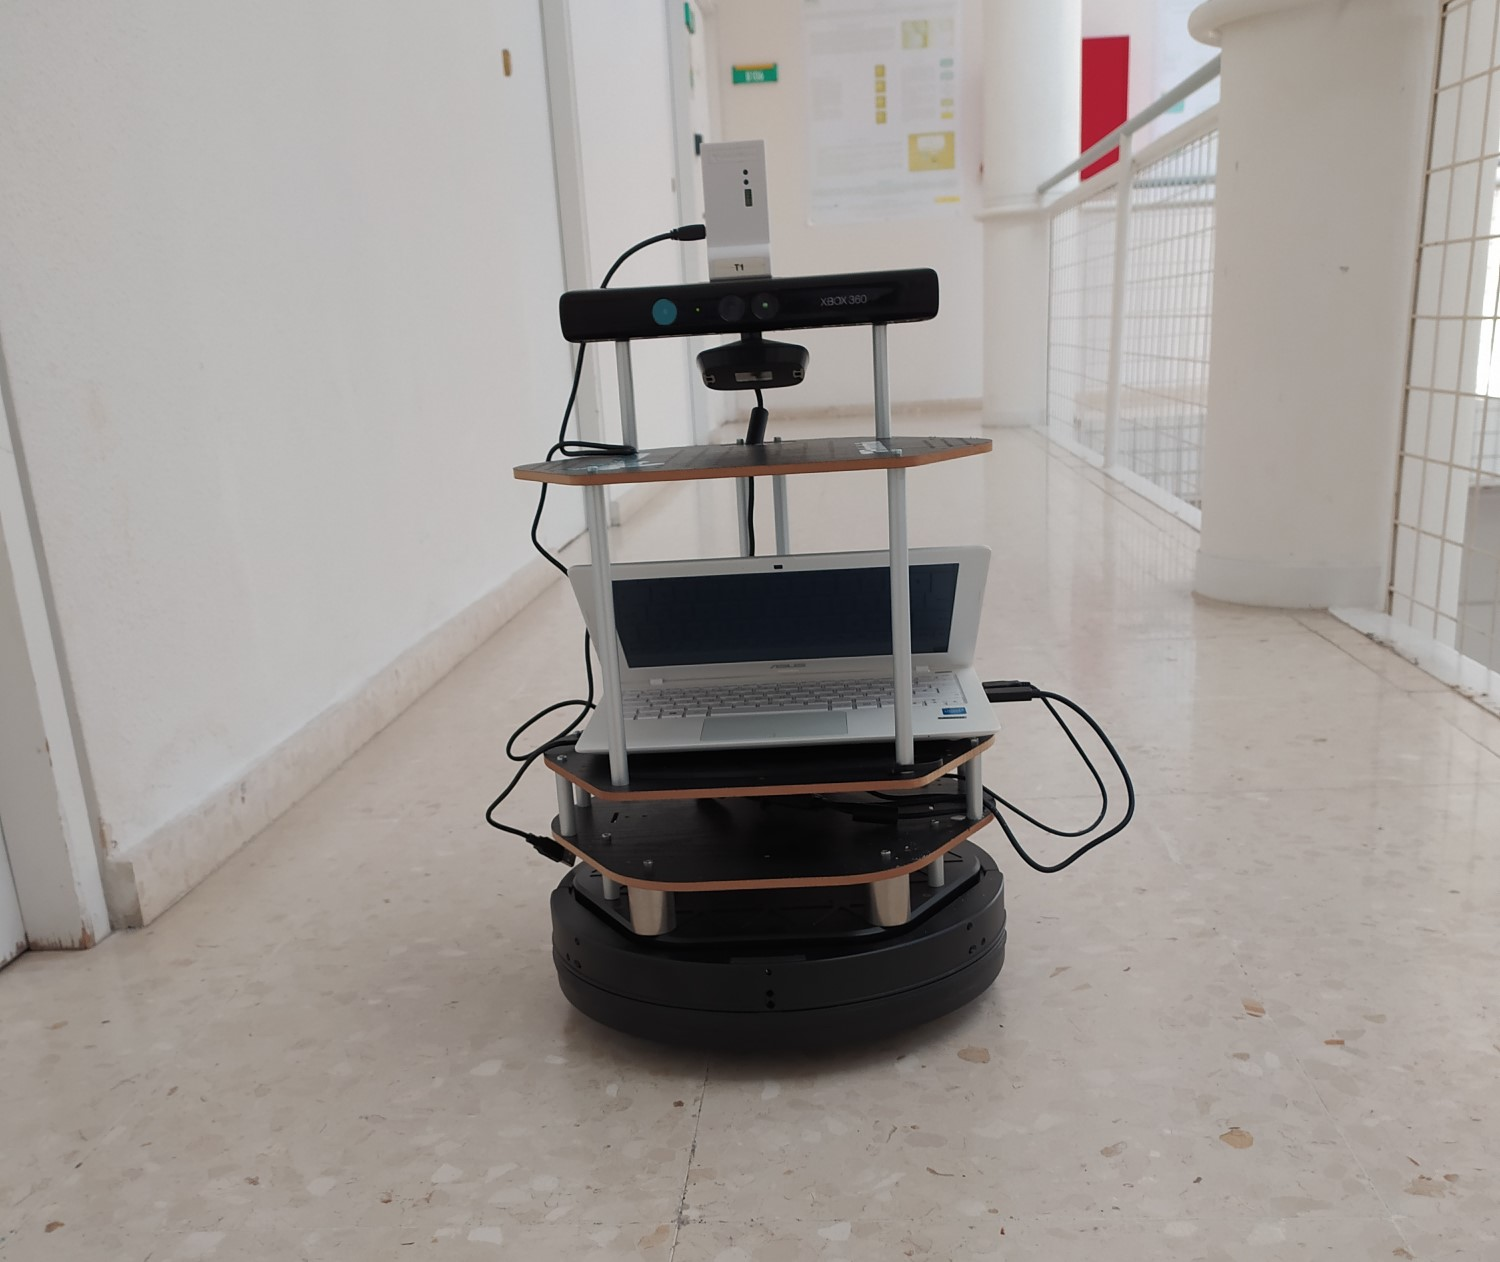
\includegraphics[width=0.75\textwidth]{pic/robot_fisica.jpg}
    \caption{Turtlebot en una de las tomas de medidas.}
    \label{fig:robot}
\end{figure}

El TurtleBot funciona con ROS --Robot Operating System, en inglés--, un entorno de trabajo enfocado a los sistemas robóticos encargado del soporte para todos los dispositivos hardware del robot como motores, encoders o cámaras. 
Cuenta con diversas librerías para distintos casos de uso, entre las que se encuentra la navegación en un entorno controlado como la que se da en el caso de este trabajo.

Dentro de los paquetes disponibles, el usado en el desarrollo del trabajo es el encargado de la navegación del robot, que permite desplazar al robot a cualquier punto del entorno.

Es posible acoplar al robot un sistema de visión que, mediante luz estructura, permite obtener un mapa de profundidad, llamado Kinect, desarrollado en primera instancia para el uso en videojuegos pero con uso también en labores de investigación al permitir el posicionamiento de objetos y paredes respecto al dicho sistema, de tal manera que permite evitar obstáculos dinámicos en el caso de que interpongan en su camino.

La funcionalidad de navegación aprovecha estos sensores realizando una fusión de sus resultados con los datos de movimiento de los motores que realizan el movimiento de tal forma que es posible corregir cualquier error en casos donde el movimiento de las ruedas no se traslade directamente en movimiento del robot, como puede ocurrir al rotar sobre sí mismo.

Para conseguir el posicionamiento en el mapa el paquete de navegación construye un \textit{planner} global sobre el que es posible determinar las rutas a seguir por el robot para llegar a un punto dado sorteando obstáculos y paredes.
Junto a él trabaja un \textit{planner} local, en el que gracias a los sensores incorporados se evalúan de forma continua los alrededores del robot.
Así, es posible conseguir de forma continua una evaluación de los posibles obstáculos que no se encuentran en el mapa del planner global, para lo que se construye un mapa de costes con el fin de abortar el movimiento en el caso de que sea imposible alcanzar el punto objetivo.

Con la información actualizada del \textit{planner} local, el \textit{planner} global es capaz de proporcionar la posición del robot en el mapa.
Es posible observar un esquema del funcionamiento de estos sistemas en la Figura~\ref{fig:move_base}.

\begin{figure}[H]
    \centering
    \def\svgwidth{0.8\linewidth}
    \input{./fig/navigation.pdf_tex}
	\caption{Esquema del funcionamiento del paquete de navegación de ROS.}
    \label{fig:move_base}
\end{figure}

Con esta herramienta la librería de navegación permite un mapeado autónomo tomando como referencia los datos de odometría que proporcionan los motores propulsores del robot para determinar las dimensiones del entorno.

En el caso de disponer de antemano de dichas dimensiones es posible proporcionar un mapa al sistema de navegación y evitar el paso de reconocimiento del entorno.
Esto no solo ahorra tiempo, sino que además minimiza las posibles discrepancias entre los datos de odometría y los desplazamientos reales del robot al realizar el mapeado de forma autónoma.

La opción de realizar un mapa previo fue la elegida en este caso, ya que el robot cuenta con rutinas para el reposicionamiento en el mapa en dicho caso.
Así, a partir de los límites establecidos y comprobados de forma manual, las posibles discrepancias en la odometría del robot se ven continuamente compensadas y corregidas.

Para facilitar el uso de ROS existe la posibilidad de usar el simulador Stage, capaz de crear un mundo virtual a partir de un mapa en dos dimensiones en el que colocar el Turtlebot y simular su funcionamiento de forma total sin tener acceso al robot de forma física.
Es posible observar su interfaz en la Figura~\ref{fig:stage_rviz}.

Además, ROS también permite el uso de una herramienta de visualización de la posición del robot en el mapa y de todos los sensores que incorpora llamada \textit{rviz}.
Aunque es compatible con Stage, sus funcionalidades brillan al usar el robot en entornos reales, donde es posible comprobar de forma continua que su posicionamiento es correcto y que sus sensores funcionan como es debido.

\begin{figure}[H]
    \centering
    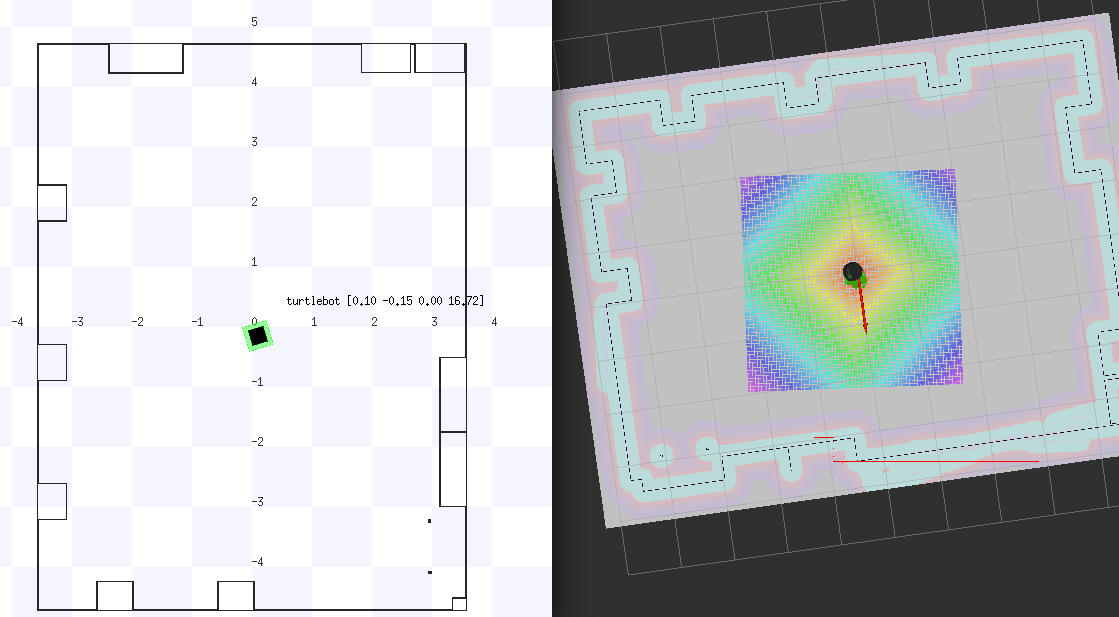
\includegraphics[width=0.75\textwidth]{pic/Stage-rviz.png}
    \caption{Captura del simulador Stage (a la izquierda) y la herramienta de visualización \textit{rviz} (a la derecha).}
    \label{fig:stage_rviz}
\end{figure}

\subsection{Sensores UWB}

Aunque el uso de UWB para el posicionamiento no está, al escribir este trabajo, utilizado de forma masiva, existen varias implementaciones comerciales que hacen uso de las técnicas geométricas mencionadas en secciones anteriores.
A pesar de que el uso de sensores propios es habitual, la adaptación de teléfonos móviles para la estimación de la posición también ha sido explorada por empresas como BeSpoon, a la espera de una implantación mayoritaria de hardware compatible en el diseño de estos dispositivos.

Los sensores utilizados han sido los pertenecientes al kit MDEK1001 ofertado por la empresa DecaWave.
Se trata de un sistema que ofrece, con una configuración mínima, la posibilidad de usar cualquiera de los componentes como baliza u objetivo.
Además, implementa un algoritmo de posicionamiento con al menos tres balizas de, según el fabricante, hasta 10cm de precisión con visión directa \cite{Decawave}.

Este kit está formado por los módulos de desarrollo DW1001, encapsulados en una carcasa de plástico que permite colocarlos encima de una superficie plana o su colocación en paredes, como se puede observar en la Figura~\ref{fig:sensor_UWB}.
Permiten obtener una alimentación a partir de baterías, como fue el uso en este trabajo para las balizas, o a partir de alimentación a través del puerto USB utilizado para la recolección de datos.

\begin{figure}[H]
    \centering
    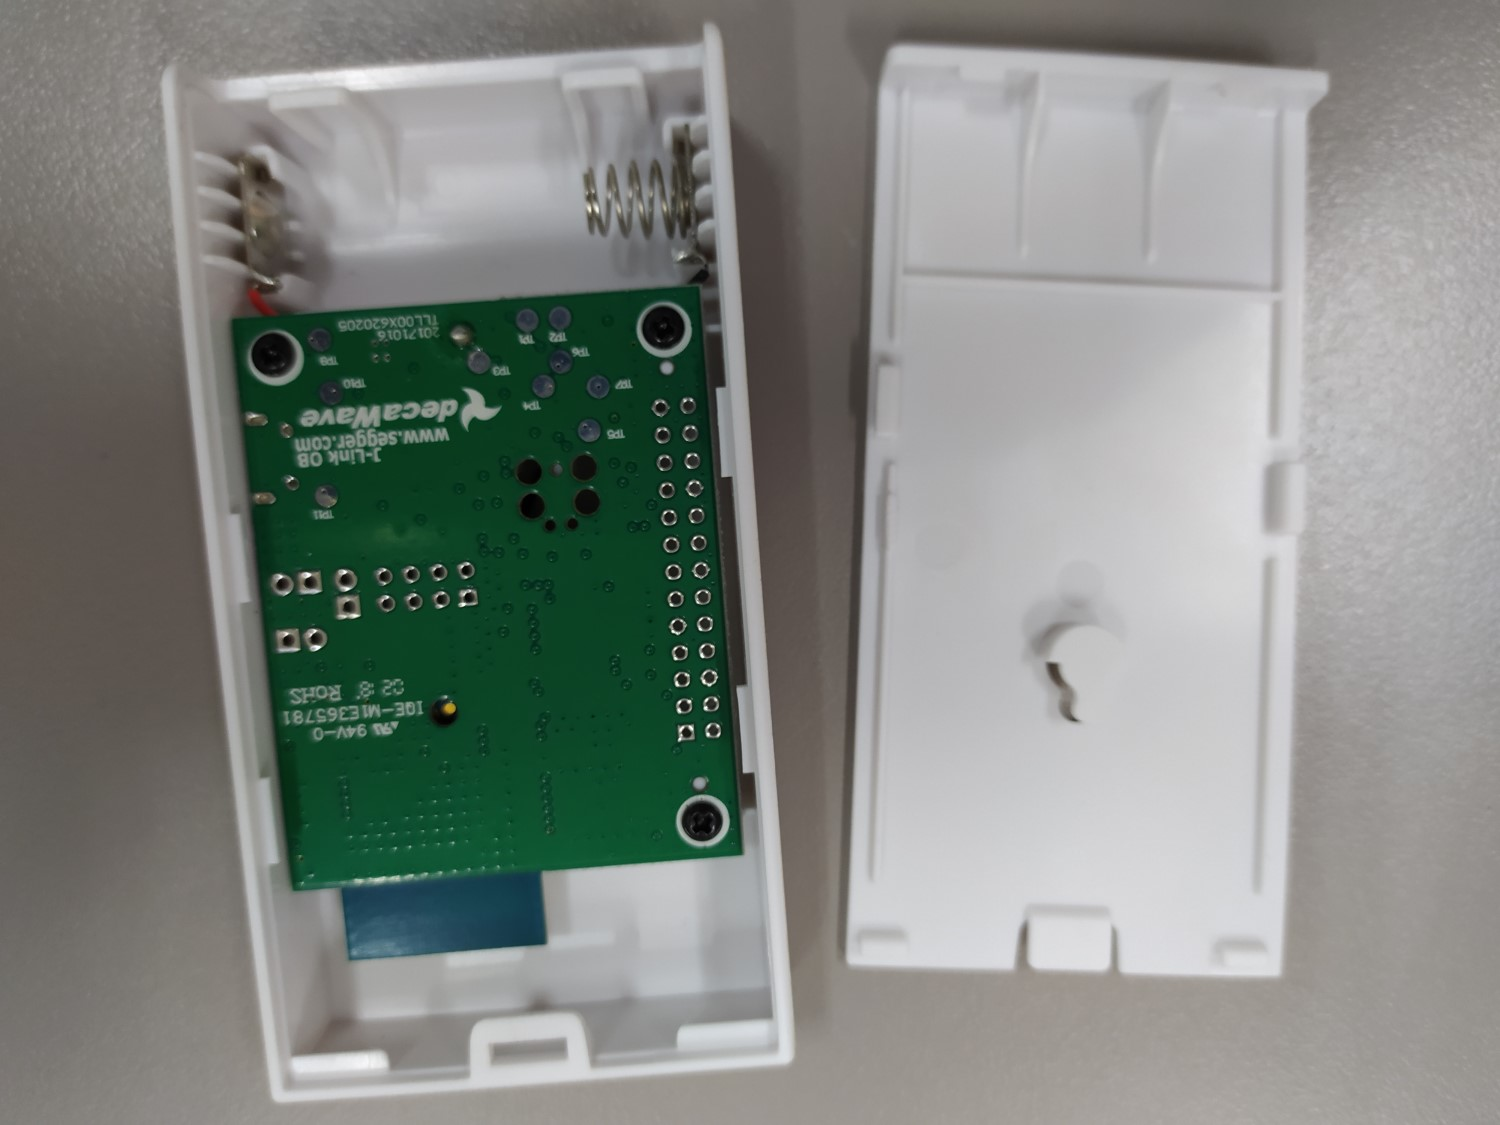
\includegraphics[width=0.65\textwidth]{pic/sensor_abierto.jpg}
    \caption{Módulo de sensor UWB DWM1001 dentro de la carcasa que lo contiene.}
    \label{fig:sensor_UWB}
\end{figure}

Algunas alternativas comerciales cuentan con antenas direccionales que permiten usar técnicas de AOA, pero no es el caso del kit utilizado que solo permite el posicionamiento con TOA y TDOA.

Los sensores, además de la comunicación por UWB, también permiten la comunicación por Bluetooth para su configuración como objetivos o balizas y en este último caso, la posición que ocupan.
También permite configurar estas posiciones de las balizas de forma automática, aunque requiere que todas se coloquen en el mismo plano y en general una configuración manual proporcionará unos mejores resultados.

Para la comunicación por UWB los sensores utilizan el canal 5, con frecuencia central de $6,5$GHz y ancho de banda de $499.2$MHz que le permiten una tasa de datos de $6.81$Mbps \cite{Decawave}.

El inicio de comercialización de dicho kit se remonta a 2017, por lo que no existe una amplia bibliografía sobre su uso en entornos reales más allá de los datos proporcionados por el fabricante.

En trabajos anteriores es posible encontrar mediciones tanto en entornos sin obstáculos con distancias bajas, en las que la precisión se encuentra en torno a los 18cm \cite{Simedroni}; como en escenarios con distancias amplias y ciertas situaciones sin línea de visión directa, donde la discrepancias crecen hasta unos 50cm \cite{jimenez, kulmer}.

DecaWave ofrece para su configuración y uso una aplicación para teléfonos móviles Android en la que representa en un mapa la posición de los sensores marcados como objetivos, pero también es posible una conexión a un ordenador como puerto serie.

Esta última opción permite obtener cuáles de las cuatro balizas --en el caso de que se configuren un número mayor de ellas-- se están usando en cada momento para realizar la estimación de la posición junto con la distancia calculada entre el objetivo y cada una de dichas balizas.

Además de la posición estimada, el algoritmo de posicionamiento proporciona un número entre 0 y 100 llamado «factor de calidad».
Debido a la naturaleza propietaria de este algoritmo, DecaWave no publica detalles sobre la obtención de este dato más allá de ser una comparación entre el posicionamiento obtenido con tres de las balizas y el obtenido al introducir la cuarta.

